\begin{frame}[parent={cmap:jabuti-gui},hasnext=true,hasprev=true]
\frametitle{Main functionalities}
\framesubtitle{File Menu}
\label{concept:file-menu}

\begin{block}{File}
The \highlight{File} menu provides options to create and manipulate a JaBUTi project.
\end{block}

\begin{block}{Demo}
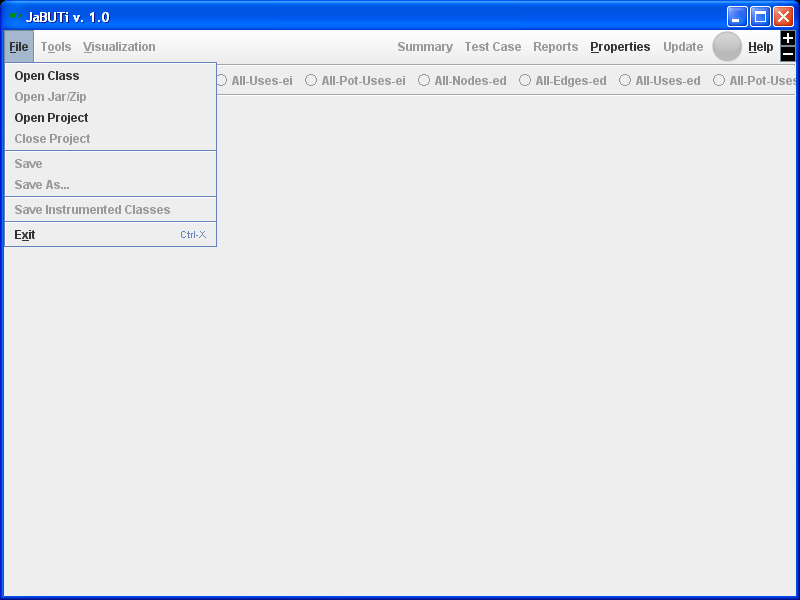
\includegraphics[width=\textwidth,clip]{JaBUTi/JaBUTi-GUI/JaBUTi-GUI-File}
\end{block}
\end{frame}



\begin{frame}
\frametitle{Main functionalities}
\framesubtitle{File Menu}
\label{concept:open-class}

\begin{block}{Open Class}
The \highlight{Open Class} menu option allows to select the base
class file from where the classes to be tested are identified.
\end{block}

\begin{block}{Demo}
\insertmovie{JaBUTi/JaBUTi-GUI/JaBUTi-GUI-File-OpenClass/JaBUTi-GUI-File-OpenClass}
\end{block}
\end{frame}



\begin{frame}
\frametitle{Main functionalities}
\framesubtitle{File Menu}
\label{concept:open-project}

\begin{block}{Open Project}
The \highlight{Open Project} option opens a previously created project.
\end{block}

\begin{block}{Demo}
\insertmovie{resources/JaBUTi/JaBUTi-GUI/JaBUTi-GUI-File-OpenProject/JaBUTi-GUI-File-OpenProject}
\end{block}
\end{frame}



\begin{frame}
\frametitle{Main functionalities}
\framesubtitle{File Menu}
\label{concept:close-project}

\begin{block}{Close Project}
The \highlight{Close Project} option closes the current project.
\end{block}

\begin{block}{Demo}
\insertmovie{JaBUTi/JaBUTi-GUI/JaBUTi-GUI-File-CloseProject/JaBUTi-GUI-File-CloseProject}
\end{block}
\end{frame}



\begin{frame}
\frametitle{Main functionalities}
\framesubtitle{File Menu}
\label{concept:save}

\begin{block}{Save}
The \highlight{Save} option saves the current project.
\end{block}

\begin{block}{Demo}
\insertmovie{JaBUTi/JaBUTi-GUI/JaBUTi-GUI-File-SaveProject/JaBUTi-GUI-File-SaveProject}
\end{block}
\end{frame}



\begin{frame}
\frametitle{Main functionalities}
\framesubtitle{File Menu}
\label{concept:save-as}

\begin{block}{Save As}
The \highlight{Save As} option saves the current project with a different name.
\end{block}

\begin{block}{Demo}
\insertmovie{JaBUTi/JaBUTi-GUI/JaBUTi-GUI-File-SaveAs/JaBUTi-GUI-File-SaveAs}
\end{block}
\end{frame}



\begin{frame}
\frametitle{Main functionalities}
\framesubtitle{File Menu}
\label{concept:save-instrumented-classes}

\begin{block}{Save Instrumented Classes}
The \highlight{Save Instrumented Classes} option saves the classes from the
current project, already instrumented for testing in production or a different
context.
\end{block}

\begin{block}{Demo}
\insertmovie{JaBUTi/JaBUTi-GUI/JaBUTi-GUI-File-SaveInstrumentedClasses/JaBUTi-GUI-File-SaveInstrumentedClasses}
\end{block}
\end{frame}



\begin{frame}
\frametitle{Main functionalities}
\framesubtitle{File Menu}
\label{concept:exit}

\begin{block}{Exit}
The \highlight{Exit} option exits of the tool.
\end{block}

\begin{block}{Demo}
\insertmovie{JaBUTi/JaBUTi-GUI/JaBUTi-GUI-File-Exit/JaBUTi-GUI-File-Exit}
\end{block}
\end{frame}
